
\subsection{A witness-oriented approach}


\begin{frame}[fragile]
\frametitle{A witness-oriented approach}

Subset-mode often works in practice, but does not seem ideal
\begin{itemize}
\item Strange normal form that affects all booleans
\item Strange iff-rewrites needed for all UBDD-making functions
\item Free variables in transitivity and the preservation of membership
\item Rules about \Code{q-ite} seem somehow fragile
\end{itemize}

\SmallSkip
\Highlight{Witness-mode} is a more advanced alternative
\begin{itemize}
\item Intuitively, ``Pick all of the probably-relevant points''
\item Casts everything in terms of \Code{eval-bdd}
\item Works with existing normal forms
\end{itemize}
\end{frame}




\begin{frame}[fragile]
\frametitle{The witness approach, graphically}

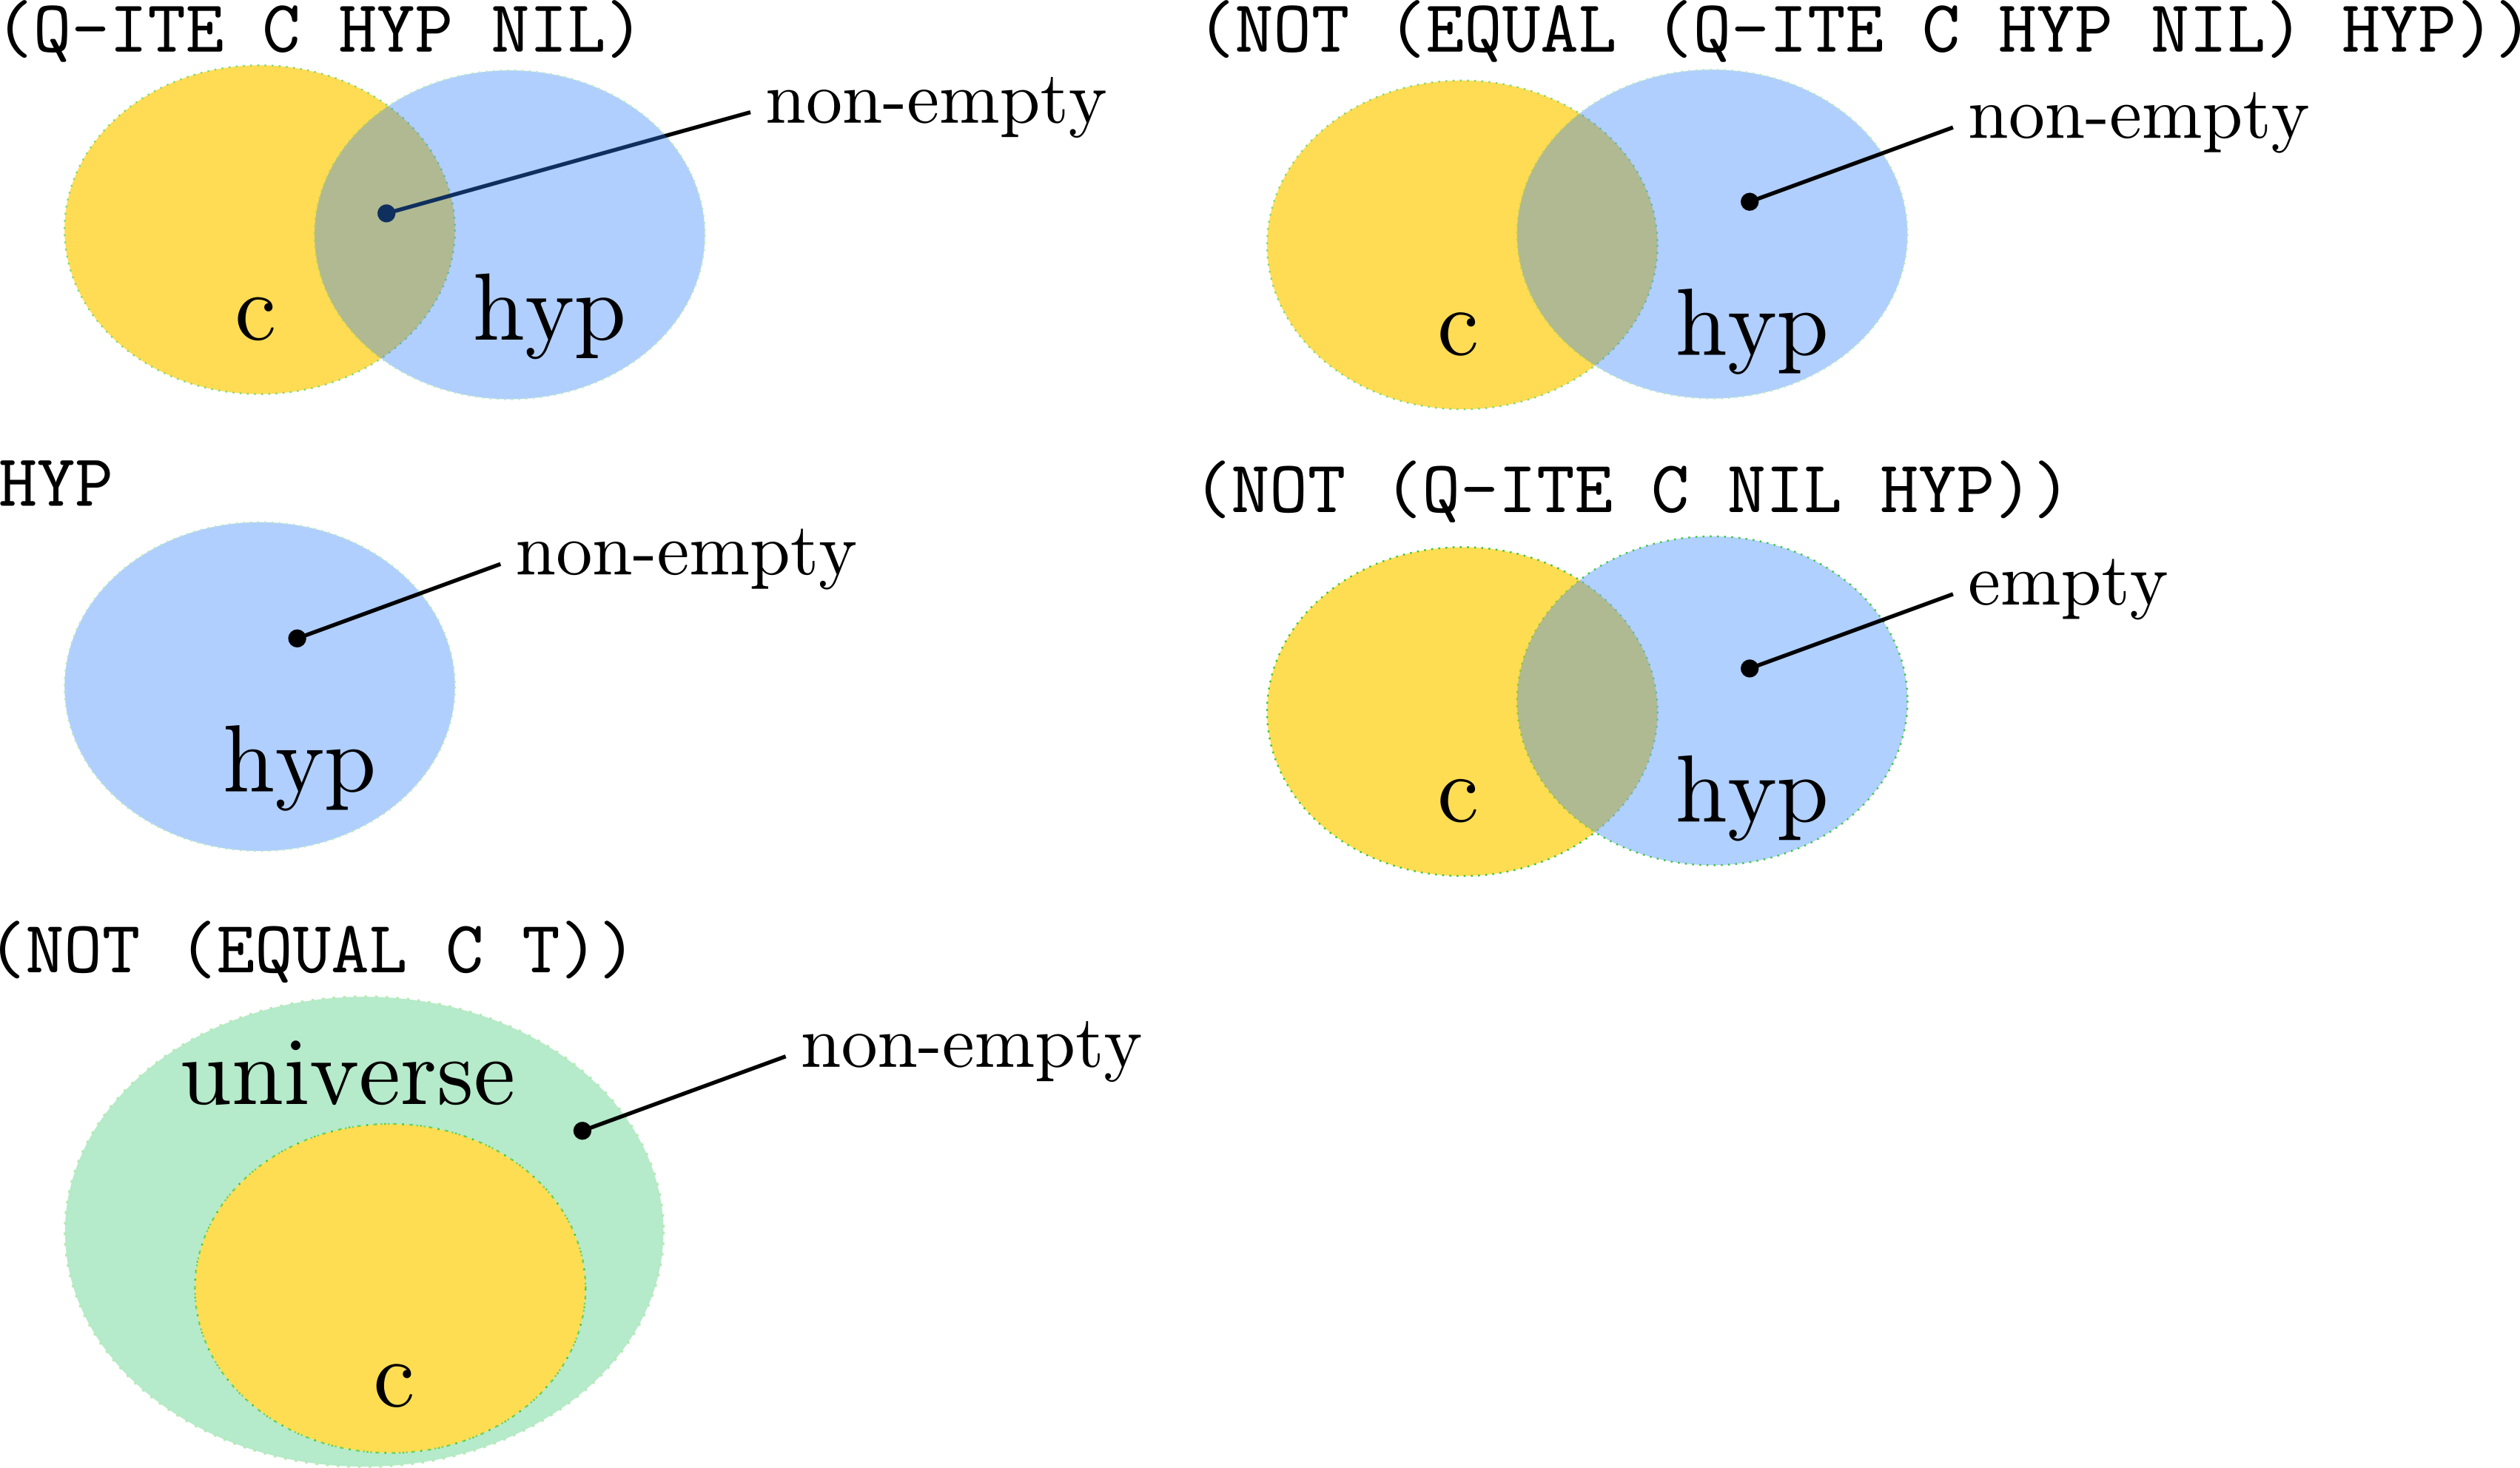
\includegraphics[width=12cm]{venn-diagrams}

\end{frame}


\begin{frame}[fragile]
\frametitle{The basic transformation}

Hypothesis: \Code{x} $\neq$ \Code{y}  (or \Code{x})
\begin{itemize}
\item Means $\exists$ \Code{v} : \Code{(eval-bdd x v)} $\neq$ \Code{(eval-bdd y v)}
\item Introduce a new variable, \Code{v}
\item Replace the hyp with \Code{(eval-bdd x v)} $\neq$ \Code{(eval-bdd y v)} 
\end{itemize}

\SmallSkip

Hypothesis: \Code{x} $=$ \Code{y}   (or \Code{(not x)})
\begin{itemize}
\item Means $\forall$ \Code{v} : \Code{(eval-bdd x v)} $=$ \Code{(eval-bdd y v)} 
\item Collect all \Code{v} occurring in the clause
\item Replace the hyp with \Code{(eval-bdd x v)} $=$ \Code{(eval-bdd y v)} 
\end{itemize}

\end{frame}


\begin{frame}[fragile]
\frametitle{Transformation example}

\begin{verbatim}
  (IMPLIES (AND ;; (NORMP C)
                ;; (NORMP HYP)
                (Q-ITE C HYP NIL)
                (NOT (EQUAL (Q-ITE C HYP NIL) HYP))
                HYP
                (NOT (EQUAL C T))
                (NOT (Q-ITE C NIL HYP))
                (NOT (EVAL-BDD C ARBITRARY-VALUES)))
           (NOT (EVAL-BDD HYP ARBITRARY-VALUES))))
\end{verbatim}

\end{frame}


\begin{frame}[fragile]

\begin{verbatim}
  (IMPLIES (AND (NOT (EQUAL (EVAL-BDD (Q-ITE C HYP NIL) V1)
                            (EVAL-BDD NIL V1)))
                (NOT (EQUAL (EVAL-BDD (Q-ITE C HYP NIL) V2)
                            (EVAL-BDD HYP V2)))
                (NOT (EQUAL (EVAL-BDD HYP V3)
                            (EVAL-BDD NIL V3)))
                (NOT (EQUAL (EVAL-BDD C V4)
                            (EVAL-BDD T V4)))
                (NOT (Q-ITE C NIL HYP))
                (NOT (EVAL-BDD C ARBITRARY-VALUES)))
           (NOT (EVAL-BDD HYP ARBITRARY-VALUES))))
\end{verbatim}

Values: \Code{V1}, \Code{V2}, \Code{V3}, \Code{V4}, \Code{ARBITRARY-VALUES}

\end{frame}


\begin{frame}[fragile]

{\footnotesize \begin{verbatim}
  (IMPLIES (AND (NOT (EQUAL (EVAL-BDD (Q-ITE C HYP NIL) V1)
                            (EVAL-BDD NIL V1)))
                (NOT (EQUAL (EVAL-BDD (Q-ITE C HYP NIL) V2)
                            (EVAL-BDD HYP V2)))
                (NOT (EQUAL (EVAL-BDD HYP V3)
                            (EVAL-BDD NIL V3)))
                (NOT (EQUAL (EVAL-BDD C V4)
                            (EVAL-BDD T V4)))

                (EQUAL (EVAL-BDD (Q-ITE C NIL HYP) V1)
                       (EVAL-BDD NIL V1))
                (EQUAL (EVAL-BDD (Q-ITE C NIL HYP) V2)
                       (EVAL-BDD NIL V2))
                (EQUAL (EVAL-BDD (Q-ITE C NIL HYP) V3)
                       (EVAL-BDD NIL V3))
                (EQUAL (EVAL-BDD (Q-ITE C NIL HYP) V4)
                       (EVAL-BDD NIL V4))
                (EQUAL (EVAL-BDD (Q-ITE C NIL HYP) ARBITRARY-VALUES)
                       (EVAL-BDD NIL ARBITRARY-VALUES))

                (NOT (EVAL-BDD C ARBITRARY-VALUES)))
           (NOT (EVAL-BDD HYP ARBITRARY-VALUES))))
\end{verbatim}}

\end{frame}


\begin{frame}[fragile]

{\small \begin{verbatim}
  (IMPLIES (AND (EVAL-BDD (Q-ITE C HYP NIL) V1)
                (NOT (EQUAL (EVAL-BDD (Q-ITE C HYP NIL) V2)
                            (EVAL-BDD HYP V2)))
                (EVAL-BDD HYP V3)
                (NOT (EVAL-BDD C V4))

                (NOT (EVAL-BDD (Q-ITE C NIL HYP) V1))
                (NOT (EVAL-BDD (Q-ITE C NIL HYP) V2))
                (NOT (EVAL-BDD (Q-ITE C NIL HYP) V3))
                (NOT (EVAL-BDD (Q-ITE C NIL HYP) V4))
                (NOT (EVAL-BDD (Q-ITE C NIL HYP) ARBITRARY-VALUES))

                (NOT (EVAL-BDD C ARBITRARY-VALUES)))
           (NOT (EVAL-BDD HYP ARBITRARY-VALUES))))
\end{verbatim}}

Follows from cases introduced by \Code{eval-bdd-of-q-ite}

\end{frame}


\begin{frame}[fragile]
\frametitle{The {\tt eval-bdd-cp} clause processor (1/2)}

\Code{(diff x y)}
\begin{itemize}
\item When \Code{x} $\neq$ \Code{y},
       \Code{(eval-bdd x (diff x y))} $\neq$ \Code{(eval-bdd y (diff x y))}
\end{itemize}

\SmallSkip
{\bf 1a.}.  Gather hyps of the form \Code{x} $\neq$ \Code{y}, where
\Code{x}, \Code{y} are (likely) UBDDs
\begin{itemize}
\item A hyp which is just \Code{x} also counts: \Code{x} $\neq$ \Code{NIL}
\end{itemize}

\SmallSkip
{\bf 1b.}.  For each \Code{x} $\neq$ \Code{y} found, replace the hyp with
\begin{center}
\Code{(implies (and (normp x) (normp y))) \qquad \qquad \qquad \qquad \qquad \qquad \quad \;} \\
\qquad \Code{(eval-bdd x (diff x y))} $\neq$ \Code{(eval-bdd y (diff x y))}
\end{center}

This is sound
\begin{itemize}
\item In the \Code{normp} case, the clauses are equivalent
\item Otherwise, the new clause implies the original
\end{itemize}

\end{frame}


\begin{frame}[fragile]
\frametitle{The {\tt eval-bdd-cp} clause processor (2/2)}

{\bf 2.} As a convenience, generalize away all \Code{(diff x y)} terms just
introduced with fresh variables. (trivially sound)

\SmallSkip
{\bf 3.} Gather up all \Code{v} which are used, anywhere, as arguments to
\Code{eval-bdd}, i.e., \Code{(eval-bdd x v)}.

\SmallSkip
{\bf 4a.} Gather hyps of the form \Code{x} $=$ \Code{y} found, where \Code{x},
\Code{y} are (likely) UBDDs
\begin{itemize}
\item A hyp which is \Code{(not x)} also counts: \Code{x} $=$ \Code{NIL}
\end{itemize}

\SmallSkip
{\bf 4b.} Replace these hyps with \Code{(eval-bdd x v)} $=$ \Code{(eval-bdd y v)}, 
for all \Code{v} found in step 3. (trivially sound)

\end{frame}



\begin{frame}[fragile]
\frametitle{Automating {\tt eval-bdd-cp}}

We use a default hint

\begin{itemize}
\item The clause must be \Code{stable-under-simplificationp}
\item The definition of \Code{eval-bdd-cp-hint} must be enabled
\item The transformation must modify the clause
\end{itemize}

\SmallSkip
The hint we give
\begin{verbatim}
(:or (:clause-processor ...)
     (:no-op t))
\end{verbatim}

\end{frame}
